\documentclass[10pt,leqno]{article}

\usepackage[%
  tmargin=1.2in,bmargin=1.2in,%
  lmargin=1.8in,rmargin=1.8in,%
]{geometry}
\usepackage{fancyhdr}
\usepackage{titlesec}
\usepackage{appendix}
\usepackage{microtype}
\usepackage[hyphens]{url}
\usepackage{enumitem}
\usepackage{xspace}
\usepackage{etoolbox}
\usepackage{ifthen}
\usepackage{tikz}
\usepackage{tikz-cd}

\usepackage{amsmath}
\definecolor{darkred}{rgb}{0.5,0.0,0.0}
\usepackage[%
  colorlinks,%
  linkcolor=darkred,%
  citecolor=darkred,%
  urlcolor=darkred,%
]{hyperref}
\usepackage{amsthm,amssymb}
% \usepackage[lining,semibold]{libertine}
% \usepackage{textcomp,stmaryrd}
% \usepackage[libertine,cmintegrals,bigdelims]{newtxmath}
% \useosf
% \usepackage[%
%   cal=boondox, calscaled=0.97,%
%   bb=boondox, bbscaled=0.98,%
% ]{mathalfa}
\usepackage{cleveref}

\frenchspacing
\urlstyle{rm}

\AtBeginDocument{%
  \setlength{\abovedisplayskip}{1.5ex plus 0.3ex minus 0.3ex}%
  \setlength{\abovedisplayshortskip}{1.0ex plus 0.3ex minus 0.3ex}%
  \setlength{\belowdisplayskip}{1.5ex plus 0.3ex minus 0.3ex}%
  \setlength{\belowdisplayshortskip}{1.0ex plus 0.3ex minus 0.3ex}%
}

\let\theoldbibliography\thebibliography
\renewcommand{\thebibliography}[1]{%
  \theoldbibliography{#1}%
  \setlength{\parskip}{0ex}
  \setlength{\itemsep}{0.5ex plus 0.2ex minus 0.2ex}
  \small
}

\pagestyle{fancy}
\renewcommand{\headrulewidth}{0pt}
\renewcommand{\footrulewidth}{0pt}
\fancyhf{}
\fancyfoot[C]{\small\thepage}

\renewcommand{\title}[1]{\newcommand{\thetitle}{#1}}
\renewcommand{\author}[1]{\newcommand{\theauthor}{#1}}
\renewcommand{\date}[1]{\newcommand{\thedate}{#1}}

\renewcommand{\maketitle}{%
  \begin{center}
    {\bfseries\MakeUppercase{%
      \thetitle}}\\[2.5ex]
    {\footnotesize\MakeUppercase{%
      \theauthor}}\\[2.5ex]
    \ifthenelse{\equal{\thedate}{}}{}{%
      \small%
      \setlength{\tabcolsep}{0.2em}%
      \begin{tabular}{rl}
        original: & \thedate \\
        updated: & \today
      \end{tabular}
    }
  \end{center}
  \vspace{2.5ex}
  \thispagestyle{fancy}
}

%%%%%%%%%%%%%%%%%%%%%%%%%%%%%%%%%%%%%%%%%%%%%%%%%%%%%%%%%%%%%%%%%%%%%%

\cspreto{section}{\setcounter{equation}{0}}

\titleformat{\section}{\centering\scshape}{\thesection.}{0.4em}{}
\titlespacing{\section}{0pt}{*4}{*1}
\titleformat{\subsection}{\scshape}{\thesubsection.}{0.4em}{}
\titlespacing{\subsection}{0pt}{*2.5}{*1}

% Display format for equations
\newcommand{\crefeqfmt}[1]{
  \crefformat{#1}{(##2##1##3)}
  \Crefformat{#1}{(##2##1##3)}
  \crefrangeformat{#1}{(##3##1##4--##5##2##6)}
  \Crefrangeformat{#1}{(##3##1##4--##5##2##6)}
  \crefmultiformat{#1}{(##2##1##3}{, ##2##1##3)}{, ##2##1##3}{, ##2##1##3)}
  \Crefmultiformat{#1}{(##2##1##3}{, ##2##1##3)}{, ##2##1##3}{, ##2##1##3)}
  \crefrangemultiformat{#1}{(##3##1##4--##5##2##6}{, ##3##1##4--##5##2##6)}{, ##3##1##4--##5##2##6}{, ##3##1##4--##5##2##6)}
  \Crefrangemultiformat{#1}{(##3##1##4--##5##2##6}{, ##3##1##4--##5##2##6)}{, ##3##1##4--##5##2##6}{, ##3##1##4--##5##2##6)}
}
% Display format for sections
\newcommand{\crefsecfmt}[1]{%
  \crefformat{#1}{\S##2##1##3}
  \Crefformat{#1}{\S##2##1##3}
  \crefrangeformat{#1}{\S\S##3##1##4--##5##2##6}
  \Crefrangeformat{#1}{\S\S##3##1##4--##5##2##6}
  \crefmultiformat{#1}{\S\S##2##1##3}{ and~##2##1##3}{, ##2##1##3}{ and~##2##1##3}
  \Crefmultiformat{#1}{\S\S##2##1##3}{ and~##2##1##3}{, ##2##1##3}{ and~##2##1##3}
  \crefrangemultiformat{#1}{\S\S##3##1##4--##5##2##6}{ and~##3##1##4--##5##2##6}{, ##3##1##4--##5##2##6}{ and~##3##1##4--##5##2##6}
  \Crefrangemultiformat{#1}{\S\S##3##1##4--##5##2##6}{ and~##3##1##4--##5##2##6}{, ##3##1##4--##5##2##6}{ and~##3##1##4--##5##2##6}
}
\crefeqfmt{equation}
\crefeqfmt{enumi}
\crefeqfmt{enumii}
\crefsecfmt{section}
\crefsecfmt{subsection}
\crefsecfmt{appendix}
\crefname{part}{Part}{Parts}
\crefname{chapter}{Chapter}{Chapters}
\crefname{figure}{Figure}{Figures}

\makeatletter

\newcommand{\thmnumfont}{\bfseries}
\newcommand{\thmheadfont}{\bfseries}
\newcommand{\thmnotefont}{\bfseries}
\newcommand{\thmhorizspace}{0.4em}

\def\swappedhead#1#2#3{%
  \thmnumber{\@upn{{\thmnumfont#2}}\@ifnotempty{#1}{.\hspace{0.25em}}}%
  \thmheadfont\thmname{#1}%
  \@ifnotempty{#3}{\ \thmnote{\thmnotefont(#3)}}%
}
\swapnumbers

\newtheoremstyle{block}%
  {2.0ex plus 0.2ex minus 0.1ex}% Space above
  {2.0ex plus 0.2ex minus 0.1ex}% Space below
  {} % Body font
  {} % Indent amount
  {\thmheadfont} % Theorem head font
  {.} % Punctuation after theorem head
  {\thmhorizspace} % Space after theorem head
  {} % Theorem head spec (can be left empty, meaning ‘normal’)

\renewenvironment{proof}[1][Proof]{\par
  \pushQED{\qed}%
  \normalfont%
  \topsep1ex plus 0.2ex minus 0.1ex\relax%
  \labelsep \thmhorizspace\relax%
  \trivlist
  \item[\hskip\labelsep\thmheadfont
    #1\@addpunct{.}]\ignorespaces
}{%
  \popQED\endtrivlist\@endpefalse%
}

\makeatother

\theoremstyle{block}

\newcommand{\defthm}[2]{%
  \newtheorem{#1}[equation]{#2}%
  \crefeqfmt{#1}%
  \newtheorem*{#1*}{#2}%
}

\defthm{algorithm}{Algorithm}
\defthm{conjecture}{Conjecture}
\defthm{construction}{Construction}
\defthm{convention}{Convention}
\defthm{corollary}{Corollary}
\defthm{definition}{Definition}
\defthm{definitions}{Definitions}
\defthm{example}{Example}
\defthm{examples}{Examples}
\defthm{exercise}{Exercise}
\defthm{fact}{Fact}
\defthm{intuition}{Intuition}
\defthm{lemma}{Lemma}
\defthm{notation}{Notation}
\defthm{nothing}{}
\defthm{proposition}{Proposition}
\defthm{question}{Question}
\defthm{remark}{Remark}
\defthm{remarks}{Remarks}
\defthm{situtation}{Situation}
\defthm{theorem}{Theorem}

\setlist{%
  leftmargin=2.5em, parsep=0ex, listparindent=\parindent,
  itemsep=1.0ex, topsep=1.0ex,%
}

\setlist[enumerate, 1]{%
  label=(\alph*),%
  ref=\alph*,%
  widest=d,%
}
\setlist[enumerate, 2]{%
  label=(\roman*),%
  ref=\theenumi.\roman*,%
}
\setlist[itemize, 1]{%
  label=$\vcenter{\hbox{\footnotesize$\bullet$}}$,%
}
\setlist[itemize, 2]{label=--}

%%%%%%%%%%%%%%%%%%%%%%%%%%%%%%%%%%%%%%%%%%%%%%%%%%%%%%%%%%%%%%%%%%%%%%

\makeatletter

\let\ea\expandafter

\newcount\foreachcount

\def\foreachletter#1#2#3{\foreachcount=#1
  \ea\loop\ea\ea\ea#3\@alph\foreachcount
  \advance\foreachcount by 1
  \ifnum\foreachcount<#2\repeat}

\def\foreachLetter#1#2#3{\foreachcount=#1
  \ea\loop\ea\ea\ea#3\@Alph\foreachcount
  \advance\foreachcount by 1
  \ifnum\foreachcount<#2\repeat}

% Roman: \rA is \mathrm{A}
\def\definerm#1{%
  \ea\gdef\csname r#1\endcsname{\ensuremath{\mathrm{#1}}\xspace}}
\foreachLetter{1}{27}{\definerm}
\foreachletter{1}{27}{\definerm}
% Script: \sA is \mathscr{A}
\def\definescr#1{%
  \ea\gdef\csname s#1\endcsname{\ensuremath{\mathscr{#1}}\xspace}}
\foreachLetter{1}{27}{\definescr}
% Calligraphic: \cA is \mathcal{A}
\def\definecal#1{%
  \ea\gdef\csname c#1\endcsname{\ensuremath{\mathcal{#1}}\xspace}}
\foreachLetter{1}{27}{\definecal}
% Bold: \bA is \mathbf{A}
\def\definebold#1{%
  \ea\gdef\csname b#1\endcsname{\ensuremath{\mathbf{#1}}\xspace}}
\foreachLetter{1}{27}{\definebold}
% Blackboard Bold: \lA is \mathbb{A}
\def\definebb#1{%
  \ea\gdef\csname l#1\endcsname{\ensuremath{\mathbb{#1}}\xspace}}
\foreachLetter{1}{27}{\definebb}
% Fraktur: \ka is \mathfrak{a}, \kA is \mathfrak{A}
\def\definefrak#1{%
  \ea\gdef\csname k#1\endcsname{\ensuremath{\mathfrak{#1}}\xspace}}
\foreachletter{1}{27}{\definefrak}
\foreachLetter{1}{27}{\definefrak}
% Sans serif: \iA \is \mathsf{A}
\def\definesf#1{%
  \ea\gdef\csname i#1\endcsname{\ensuremath{\mathsf{#1}}\xspace}}
\foreachletter{1}{6}{\definesf}
\foreachletter{7}{14}{\definesf}
\foreachletter{15}{27}{\definesf}
\foreachLetter{1}{27}{\definesf}
% Bar: \Abar is \overline{A}, \abar is \overline{a}
\def\definebar#1{%
  \ea\gdef\csname #1bar\endcsname{\ensuremath{\overline{#1}}\xspace}}
\foreachLetter{1}{27}{\definebar}
\foreachletter{1}{8}{\definebar} % \hbar is something else!
\foreachletter{9}{15}{\definebar} % \obar is something else!
\foreachletter{16}{27}{\definebar}
% Tilde: \Atil is \widetilde{A}, \atil is \widetilde{a}
\def\definetil#1{%
  \ea\gdef\csname #1til\endcsname{\ensuremath{\widetilde{#1}}\xspace}}
\foreachLetter{1}{27}{\definetil}
\foreachletter{1}{27}{\definetil}
% Hats: \Ahat is \widehat{A}, \ahat is \widehat{a}
\def\definehat#1{%
  \ea\gdef\csname #1hat\endcsname{\ensuremath{\widehat{#1}}\xspace}}
\foreachLetter{1}{27}{\definehat}
\foreachletter{1}{27}{\definehat}
% Checks: \Achk is \widecheck{A}, \achk is \widecheck{a}
\def\definechk#1{%
  \ea\gdef\csname #1chk\endcsname{\ensuremath{\widecheck{#1}}\xspace}}
\foreachLetter{1}{27}{\definechk}
\foreachletter{1}{27}{\definechk}
% Underline: \Aund is \underline{A}, \aund is \underline{a}
\def\defineul#1{%
  \ea\gdef\csname #1und\endcsname{\ensuremath{\underline{#1}}\xspace}}
\foreachLetter{1}{27}{\defineul}
\foreachletter{1}{27}{\defineul}

\makeatother

%%%%%%%%%%%%%%%%%%%%%%%%%%%%%%%%%%%%%%%%%%%%%%%%%%%%%%%%%%%%%%%%%%%%%%

\usetikzlibrary{calc,decorations.pathmorphing,shapes,arrows}
\tikzcdset{
  arrow style=tikz,
  diagrams={>={stealth}},
}

\newcommand{\arrlen}{1em}
\renewcommand{\to}{\mathrel{\tikz[baseline]%
    \draw[>=stealth,->](0,0.5ex)--(\arrlen,0.5ex);}}
\newcommand{\from}{\mathrel{\tikz[baseline]%
    \draw[>=stealth,<-](0,0.5ex)--(\arrlen,0.5ex);}}
\renewcommand{\mapsto}{\mathrel{\tikz[baseline]%
    \draw[>=stealth,|->](0,0.5ex)--(\arrlen,0.5ex);}}
\newcommand{\inj}{\mathrel{\tikz[baseline]%
    \draw[>=stealth,right hook->](0,0.5ex)--(\arrlen,0.5ex);}}
\newcommand{\surj}{\mathrel{\tikz[baseline]%
    \draw[>=stealth,->>](0,0.5ex)--(\arrlen,0.5ex);}}
\newcommand{\fromto}{\mathrel{%
  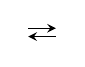
\begin{tikzpicture}[baseline]%
    \draw[>=stealth,<-](0,0.15ex)--(\arrlen,0.15ex);%
    \draw[>=stealth,->](0,0.85ex)--(\arrlen,0.85ex);%
  \end{tikzpicture}}}
\newcommand{\doubto}{\mathrel{%
  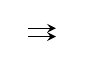
\begin{tikzpicture}[baseline]%
    \draw[>=stealth,->](0,0.15ex)--(\arrlen,0.15ex);%
    \draw[>=stealth,->](0,0.85ex)--(\arrlen,0.85ex);%
  \end{tikzpicture}}}
\newcommand{\lblto}[1]{\mathrel{%
    \begin{tikzpicture}[baseline= {( $ (current bounding box.south) + (0,-0.5ex) $ )}]
      \node[inner sep=.4ex] (a) {\,$\scriptstyle #1$\,};
      \draw[>=stealth,->] (a.south west) -- (a.south east);
    \end{tikzpicture}}}
\newcommand{\isoto}{\lblto{\sim}}

\newcommand{\simpl}[3]{
  \begin{tikzcd}[ampersand replacement=\&, column sep=small]
    #1 \&
    #2 \ar[l, shift right=0.35ex]
       \ar[l, shift left=0.35ex] \&
    #3 \ar[l, shift right=0.70ex]
       \ar[l, shift left=0.70ex]
       \ar[l] \&
    \cdots \ar[l, shift right=0.35ex]
           \ar[l, shift left=0.35ex]
           \ar[l, shift right=1.05ex]
           \ar[l, shift left=1.05ex]
  \end{tikzcd}
}
\newcommand{\cosimpl}[3]{
  \begin{tikzcd}[ampersand replacement=\&, column sep=small]
    #1 \ar[r, shift right=0.35ex]
       \ar[r, shift left=0.35ex] \&
    #2 \ar[r, shift right=0.70ex]
       \ar[r, shift left=0.70ex]
       \ar[r] \&
    #3 \ar[r, shift right=0.35ex]
       \ar[r, shift left=0.35ex]
       \ar[r, shift right=1.05ex]
       \ar[r, shift left=1.05ex] \&
    \cdots
  \end{tikzcd}
}

\newcommand{\tto}{\mathrel{\tikz[baseline]%
    \draw[>=stealth,->,double, double distance = 0.3ex](0,0.5ex)--(\arrlen,0.5ex);}}
\newcommand{\doubfrom}{\mathrel{%
  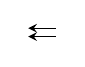
\begin{tikzpicture}[baseline]%
    \draw[>=stealth,<-](0,0.15ex)--(\arrlen,0.15ex);%
    \draw[>=stealth,<-](0,0.85ex)--(\arrlen,0.85ex);%
  \end{tikzpicture}}}
\newcommand{\tripfrom}{\mathrel{%
  
\begin{tikzpicture}[baseline]%
    \draw[>=stealth,<-](0,0.00ex)--(\arrlen,0.00ex);%
    \draw[>=stealth,<-](0,0.50ex)--(\arrlen,0.50ex);%
    \draw[>=stealth,<-](0,1.00ex)--(\arrlen,1.00ex);%
  \end{tikzpicture}}}


\renewcommand{\l}{\left}
\renewcommand{\r}{\right}
\newcommand{\f}{\frac}
\renewcommand{\o}{\overline}
\renewcommand{\u}{\underline}
\newcommand{\til}{\widetilde}
\renewcommand{\hat}{\widehat}
\newcommand{\del}{\partial}
\newcommand{\dash}{\text{-}}
\renewcommand{\c}{\colon}
\newcommand{\lc}{\,:\!}
\newcommand{\ce}{\coloneq}%{\mathrel{:=}}
\newcommand{\ec}{\eqcolon}%{\mathrel{=:}}
\newcommand{\iso}{\simeq}
\newcommand{\dual}{\vee}
\newcommand{\ldb}{\llbracket}
\newcommand{\rdb}{\rrbracket}

\newcommand{\Obj}{\operatorname{Obj}}
\newcommand{\Hom}{\operatorname{Hom}}
\newcommand{\Map}{\operatorname{Map}}
\newcommand{\Fun}{\operatorname{Fun}}
\newcommand{\Aut}{\operatorname{Aut}}
\newcommand{\Iso}{\operatorname{Iso}}
\renewcommand{\id}{\mathrm{id}}
\renewcommand{\im}{\operatorname{im}}
\newcommand{\op}{\mathrm{op}}
\newcommand{\univ}{\mathrm{univ}}
\newcommand{\colim}{\operatorname*{colim}}
\newcommand{\dlim}{\displaystyle\lim}
\newcommand{\dcolim}{\displaystyle\colim}
\newcommand{\Spec}{\operatorname{Spec}}
\newcommand{\Spf}{\operatorname{Spf}}

%%%%%%%%%%%%%%%%%%%%%%%%%%%%%%%%%%%%%%%%%%%%%%%%%%%%%%%%%%%%%%%%%%%%%%


\title{Math 216A Homework 2}
\author{Arpon Raksit}
\date{7 October 2016}

\numberwithin{block}{section}

%%%%%%%%%%%%%%%%%%%%%%%%%%%%%%%%%%%%%%%%%%%%%%%%%%%%%%%%%%%%%%%%%%%%%%


\begin{document}
\maketitle

%%%%%%%%%%%%%%%%%%%%%%%%%%%%%%%%%%%%%%%%%%%%%%%%%%%%%%%%%%%%%%%%%%%%%%

\section{Hartshorne exercise  II.2.22}

Let $X$ be a topological space and $\{U_i\}$ an open cover of $X$. Let $U_{i,j} \ce U_i \cap U_j$ (considering $(i,j)$ as an \emph{ordered} pair). Let
\[
  f_i \c U_i \inj X, \quad
  f_{i,j} \c U_{i,j} \inj X, \quad
  f^i_{i,j} \c U_{i,j} \inj U_i, \quad
  f^j_{i,j} \c U_{i,j} \inj U_i
\]
denote the inclusions.

\begin{lemma}
  \label{sheaf-recovering}
  Let $\sF$ be a sheaf on $X$. Let $\sF_i \ce (f_i)^*\sF$ and $\sF_{i,j} \ce (f_{i,j})^*\sF = (f^i_{i,j})^*\sF_i = (f^j_{i,j})^*\sF_j$. Then we have a canonical equalizer sequence of sheaves
  \[
    \sF \to \prod_i (f_i)_*\sF_i \doubto \prod_{i,j} (f_{i,j})_*\sF_{i,j},
  \]
  where here:
  \begin{itemize}
  \item the left map is given on the $i$-th factor of the target by the unit map $\sF \to (f_i)_*\sF_i = (f_i)_*(f_i)^*\sF$ of the adjunction $(f_i)^* \dashv (f_i)_*$;
  \item the upper right map is given on the $(i,j)$-th factor of the target by projection onto the $i$-th factor of the source followed by $(f_i)_*$ applied to the unit map $\sF_i \to (f^i_{i,j})_*\sF_{i,j} = (f^i_{i,j})_*(f^i_{i,j})^*\sF_i$ of the adjunction $(f^i_{i,j})^* \dashv (f^i_{i,j})_*$;
  \item the lower right map is given on the $(i,j)$-th factor of the target by projection onto the $j$-th factor of the source followed by $(f_j)_*$ applied to the unit map $\sF_j \to (f^j_{i,j})_*\sF_{i,j} = (f^j_{i,j})_*(f^j_{i,j})^*\sF_i$ of the adjunction $(f^j_{i,j})^* \dashv (f^j_{i,j})_*$.
  \end{itemize}
\end{lemma}

\begin{proof}
  Limits of sheaves are computed as limits of presheaves, so it suffices to check that the above gives an equalizer sequence after evaluating on any open set $V \subseteq X$. Well, this is precisely the sequence
  \[
    \sF(V) \to \prod_i \sF(V \cap U_i) \doubto \prod_{i,j} \sF(V \cap U_i \cap U_j)
  \]
  that the sheaf condition (applied to the cover ${V \cap U_i}$ of $V$) tells us is an equalizer.
\end{proof}

\begin{proposition}
  \label{sheaf-gluing}
  Suppose given for each $i$ a sheaf $\sF_i$ on $U_i$, and for each $(i,j)$ an isomorphism $\phi_{i,j} \c (f^i_{i,j})^*\sF_i \isoto (f^j_{i,j})^*\sF_j$, such that $\phi_{i,i}$ is the identity for each $i$ and for any $(i,j,k)$ we have $\phi_{i,k} = \phi_{j,k} \circ \phi_{i,j}$ when restricted to $U_{i,j,k} \ce U_i \cap U_j \cap U_k$. Then there exists a unique (up to unique isomorphism) sheaf $\sF$ on $X$ equipped with isomorphisms $\psi_i \c (f_i)^*\sF \isoto \sF_i$ such that $\phi_{i,j} = \psi_j \circ \psi_i^{-1}$ (restricted to $U_{i,j})$.
\end{proposition}

\begin{proof}
  Inspired by \cref{sheaf-recovering}, we will consider two maps
  \[
    \prod_i (f_i)_*\sF_i \doubto \prod_{i,j} (f_{i,j})_*\sF_{i,j},
  \]
  defined as follows:
  \begin{itemize}
  \item the upper map is just as in \cref{sheaf-recovering}, given on the $(i,j)$-th factor of the target by projection onto the $i$-th factor of the source followed by $(f_i)_*$ applied to the unit map $\sF_i \to (f^i_{i,j})_*\sF_{i,j} = (f^i_{i,j})_*(f^i_{i,j})^*\sF_i$ of the adjunction $(f^i_{i,j})^* \dashv (f^i_{i,j})_*$;
  \item the lower map is less tautological, given on the $(i,j)$-th factor of the target by projection onto the $j$-th factor of the source followed by $(f_j)_*$ applied to the map $\sF_j \to (f^j_{i,j})_*\sF_{i,j} = (f^j_{i,j})_*(f^j_{i,j})^*\sF_i$ which is adjoint to $\phi_{j,i}$ in the adjunction $(f^j_{i,j})^* \dashv (f^j_{i,j})_*$.
  \end{itemize}
  To prove existence, we will show that the equalizer of these maps supplies us with the desired $\sF$ and $\psi_i$. To prove uniqueness, we will show that any such $\sF$ and $\psi_i$ supply us with an equalizer of these two maps\footnote{This also provides a universal property for mapping into the glued sheaf.}.

  Let's begin with existence. So let $\sF$ be the equalizer of the above two maps. This gives us a canonical map $\alpha \c \sF \to \prod_i (f_i)_*\sF_i$, and we define $\psi_i \c (f_i)^*\sF \to \sF_i$ to be adjoint to the map $\alpha_i \c \sF \to (f_i)_*\sF_i$ in the $i$-th factor. That $\alpha$ equalizes the two maps above tells us precisely that for each $(i,j)$ we have $\psi_j = \phi_{i,j} \circ \psi_i$ on $U_{i,j}$. Thus we need only show for each $i$ that $\psi_i$ is an isomorphism.

  Since $f_i$ is an open inclusion, it's clear that $(f_i)^*$ preserves limits (including products and equalizers), and hence we may pull back our equalizer sequence to $U_i$:
  \[
    (f_i)^*\sF \to \prod_j (f_i)^*(f_j)_*\sF_j \doubto \prod_{j,k} (f_i)^*(f_{j,k})_*\sF_{j,k}.
  \]
  Then since $(f_i)^*(f_j)_* = (f^i_{i,j})_*(f_i)^*$ and similarly for $(f_i)^*(f_{j,k})_*$, we may reduce to the case that $U_i = X$ (and $f_i = \id_X$), and $\psi_i = \alpha_i$ is just a map $\sF \to \sF_i$.

  We define an inverse map $\beta_i \c \sF_i \to \sF$. By definition of equalizer, this means we must define a map $\beta'_i \c \sF_i \to \prod_j (f_j)_*\sF_j$ which equalizes the two maps to $\prod_{j,k} (f_{j,k})_*\sF_{j,k}$. We achieve this by defining the $j$-th factor $\beta'_{i,j}$ of $\beta'_i$ to be the map $\sF_i \to (f_j)_*\sF_j$ adjoint to the isomorphism $\phi_{j,i} \c (f_j)^*\sF_i \isoto \sF_i$; that $\beta'_i$ equalizes the two maps follows from the cocycle condition $\phi_{i,k} = \phi_{j,k} \circ \phi_{i,j}$. That $\alpha_i \circ \beta_i = \id_{\sF_i}$ is immediate from the condition that $\phi_{i,i}$ is the identity. To check $\beta_i \circ \alpha_i = \id_{\sF}$ is equivalent to checking $\alpha_j = \beta'_{i,j} \circ \alpha_i \c \sF \to (f_j)_*\sF_j$. Chasing through the definitions (note $\beta'_{i,j}$ is defined identically to the $(i,j)$-th factor of the lower map of the equalizer), this is immediate from $\alpha$ equalizing the two maps. This finishes the proof that $\alpha_i$ is an isomorphism, and hence finishes the construction.

  We now prove uniqueness. Suppose given a sheaf $\sF$ on $X$ with isomorphisms $\psi_i$ as in the statement of the proposition. Observe that this gives us a commutative diagram (or rather two overlaid commutative diagrams)
  \[
    \begin{tikzcd}
      \prod_i (f_i)_*(f_i)^*\sF \ar[r, shift left=0.5ex] \ar[r, shift right=0.5ex] \ar[d, "((f_i)_*(\psi_i))"] & 
      \prod_{i,j} (f_{i,j})_*(f_{i,j})^*\sF \ar[d, "((f_i)_*(f^i_{i,j})^*(\psi_i))"] \\
      \prod_i (f_i)_*\sF_i \ar[r, shift left=0.5ex] \ar[r, shift right=0.5ex] & 
      \prod_{i,j} (f_{i,j})_*\sF_{i,j},
    \end{tikzcd}
  \]
  where the first row is the pair of maps appearing in \cref{sheaf-recovering} and the second row is the pair we've been considering in this proof. By \cref{sheaf-recovering} $\sF$ is an equalizer of the top row. Since the vertical maps are isomorphisms, it must be an equalizer of the bottom row as well.
\end{proof}

%%%%%%%%%%%%%%%%%%%%%%%%%%%%%%%%%%%%%%%%%%%%%%%%%%%%%%%%%%%%%%%%%%%%%%

\end{document}
